\documentclass{article}

\usepackage{inputenc}
\usepackage{csquotes}
\usepackage[a4paper, total={6in, 10in}]{geometry}
\usepackage{hyperref}
\usepackage{amsmath,amssymb}
\usepackage{graphicx}
\usepackage{indentfirst}
\usepackage{caption}
\usepackage{subcaption}
\usepackage[
singlelinecheck=false % <-- important
]{caption}
\usepackage{float}
\usepackage{booktabs}
\begin{document}

\begin{table}[h!] \centering
   \caption{Main table}
   {
\def\sym#1{\ifmmode^{#1}\else\(^{#1}\)\fi}
\begin{tabular}{l*{3}{c}}
\hline\hline
          &\multicolumn{1}{c}{(1)}&\multicolumn{1}{c}{(2)}&\multicolumn{1}{c}{(3)}\\
          &\multicolumn{1}{c}{D.ln\_med\_rent\_psqft}&\multicolumn{1}{c}{D.ln\_med\_rent\_psqft}&\multicolumn{1}{c}{D.ln\_med\_rent\_psqft}\\
\hline
D.ln\_mw   &   0.0260\sym{**} &   0.0257\sym{**} &   0.0255\sym{**} \\
          & (0.0128)         & (0.0120)         & (0.0117)         \\
\hline
Zipcode-specifc linear trend&       No         &      Yes         &      Yes         \\
Zipcode-specific linear and square trend&       No         &       No         &      Yes         \\
R-squared &    0.022         &    0.024         &    0.026         \\
Observations&   112232         &   112232         &   112232         \\
\hline\hline
\end{tabular}
}

\end{table}

\begin{table}[h!] \centering
	\caption{Polynomial trends}
	{
\def\sym#1{\ifmmode^{#1}\else\(^{#1}\)\fi}
\begin{tabular}{l*{3}{c}}
\hline\hline
          &\multicolumn{1}{c}{(1)}         &\multicolumn{1}{c}{(2)}         &\multicolumn{1}{c}{(3)}         \\
\hline
$\Delta \ln \underline{w}_{it}$&    0.026\sym{*}  &    0.026\sym{**} &    0.025\sym{**} \\
          &  (0.013)         &  (0.012)         &  (0.012)         \\
\hline
Zipcode-specifc linear trend&       No         &      Yes         &      Yes         \\
Zipcode-specific quadratic trend&       No         &       No         &      Yes         \\
R-squared &    0.022         &    0.024         &    0.026         \\
Observations&  112,232         &  112,232         &  112,232         \\
\hline\hline
\end{tabular}
}

\end{table}

\clearpage
\begin{table}[h!] \centering
	\caption{Dynamic models}
	{
\def\sym#1{\ifmmode^{#1}\else\(^{#1}\)\fi}
\begin{tabular}{l*{4}{c}}
\hline\hline
          &\multicolumn{1}{c}{(1)}&\multicolumn{1}{c}{(2)}&\multicolumn{1}{c}{(3)}&\multicolumn{1}{c}{(4)}\\
          &\multicolumn{1}{c}{D.ln\_medrentpricepsqft\_sfcc}&\multicolumn{1}{c}{D.ln\_medrentpricepsqft\_sfcc}&\multicolumn{1}{c}{D.ln\_medrentpricepsqft\_sfcc}&\multicolumn{1}{c}{D.ln\_medrentpricepsqft\_sfcc}\\
\hline
F6D.ln\_actual\_mw& -0.00700         & -0.00723         & -0.00803         & -0.00753         \\
          &(0.00788)         &(0.00683)         &(0.00689)         &(0.00702)         \\
[1em]
F5D.ln\_actual\_mw&  -0.0113         &  -0.0119         &  -0.0133         &  -0.0122         \\
          &(0.00973)         & (0.0106)         & (0.0104)         & (0.0108)         \\
[1em]
F4D.ln\_actual\_mw& -0.00451         & -0.00508         & -0.00658         & -0.00546         \\
          & (0.0122)         & (0.0113)         & (0.0113)         & (0.0106)         \\
[1em]
F3D.ln\_actual\_mw&  0.00261         &  0.00200         & 0.000518         &  0.00163         \\
          & (0.0114)         & (0.0114)         & (0.0111)         & (0.0116)         \\
[1em]
F2D.ln\_actual\_mw&  0.00404         &  0.00344         &  0.00194         &  0.00314         \\
          & (0.0131)         & (0.0127)         & (0.0130)         & (0.0126)         \\
[1em]
FD.ln\_actual\_mw& -0.00353         & -0.00404         & -0.00560         & -0.00482         \\
          & (0.0109)         & (0.0130)         & (0.0127)         & (0.0134)         \\
[1em]
D.ln\_actual\_mw&   0.0307\sym{**} &   0.0299\sym{**} &   0.0278\sym{**} &   0.0287\sym{**} \\
          & (0.0138)         & (0.0116)         & (0.0120)         & (0.0119)         \\
[1em]
LD.ln\_actual\_mw&   0.0127\sym{**} &   0.0118\sym{*}  &  0.00977         &   0.0108         \\
          &(0.00565)         &(0.00595)         &(0.00586)         &(0.00665)         \\
[1em]
L2D.ln\_actual\_mw& -0.00782         & -0.00877         &  -0.0108         & -0.00976         \\
          & (0.0136)         & (0.0121)         & (0.0122)         & (0.0123)         \\
[1em]
L3D.ln\_actual\_mw&  0.00680         &  0.00583         &  0.00387         &  0.00491         \\
          &(0.00851)         &(0.00745)         &(0.00794)         &(0.00855)         \\
[1em]
L4D.ln\_actual\_mw&   0.0104         &  0.00951         &  0.00788         &  0.00876         \\
          &(0.00741)         &(0.00725)         &(0.00713)         &(0.00809)         \\
[1em]
L5D.ln\_actual\_mw&  0.00913         &  0.00823         &  0.00664         &  0.00749         \\
          &(0.00672)         &(0.00711)         &(0.00693)         &(0.00705)         \\
[1em]
L6D.ln\_actual\_mw&  0.00378         &  0.00394         &  0.00273         &  0.00311         \\
          & (0.0121)         & (0.0117)         & (0.0119)         & (0.0115)         \\
\hline
Zipcode-specifc linear trend&       No         &      Yes         &      Yes         &      Yes         \\
Zipcode-specific linear and square trend&       No         &       No         &      Yes         &      Yes         \\
Zipcode-specific linear, square and cubic trend&       No         &       No         &       No         &      Yes         \\
R-squared & .0224817         & .0245459         & .0267439         & .0290873         \\
Observations&   102078         &   102078         &   102078         &   102078         \\
\hline\hline
\end{tabular}
}

\end{table}


\clearpage
\begin{table}[h!] \centering
	\caption{Horse race models}
	\resizebox{\textwidth}{!}{
		{
\def\sym#1{\ifmmode^{#1}\else\(^{#1}\)\fi}
\begin{tabular}{l*{7}{c}}
\hline\hline
          &\multicolumn{1}{c}{(1)}&\multicolumn{1}{c}{(2)}&\multicolumn{1}{c}{(3)}&\multicolumn{1}{c}{(4)}&\multicolumn{1}{c}{(5)}&\multicolumn{1}{c}{(6)}&\multicolumn{1}{c}{(7)}\\
          &\multicolumn{1}{c}{DiD}&\multicolumn{1}{c}{\shortstack{Distributed \\ leads and lags}}&\multicolumn{1}{c}{\shortstack{Distributed \\ Lags}}&\multicolumn{1}{c}{\shortstack{AB Distributed \\ leads and lags}}&\multicolumn{1}{c}{\shortstack{AB Distributed \\ Lags}}&\multicolumn{1}{c}{\shortstack{MW Distributed \\ leads and lags}}&\multicolumn{1}{c}{\shortstack{MW Distributed \\ Lags}}\\
\hline
$\Delta \ln \underline{w}_{i,t-5}$&                  &  -0.0146         &                  &  -0.0134         &                  &  -0.0167         &                  \\
          &                  &(0.00910)         &                  &(0.00910)         &                  & (0.0155)         &                  \\
[1em]
$\Delta \ln \underline{w}_{i,t-4}$&                  & -0.00232         &                  &  0.00494         &                  & -0.00886         &                  \\
          &                  & (0.0116)         &                  & (0.0105)         &                  & (0.0347)         &                  \\
[1em]
$\Delta \ln \underline{w}_{i,t-3}$&                  &  0.00137         &                  &  0.00222         &                  & 0.000503         &                  \\
          &                  &(0.00931)         &                  &(0.00918)         &                  & (0.0152)         &                  \\
[1em]
$\Delta \ln \underline{w}_{i,t-2}$&                  &  0.00608         &                  &  0.00581         &                  &  0.00647         &                  \\
          &                  & (0.0115)         &                  & (0.0139)         &                  & (0.0102)         &                  \\
[1em]
$\Delta \ln \underline{w}_{i,t-1}$&                  &-0.000280         &                  & -0.00531         &                  &-0.000132         &                  \\
          &                  & (0.0123)         &                  & (0.0151)         &                  & (0.0154)         &                  \\
[1em]
$\Delta \ln \underline{w}_{i,t}$&   0.0259\sym{*}  &   0.0270\sym{**} &   0.0261\sym{*}  &   0.0294\sym{*}  &   0.0288\sym{*}  &   0.0267\sym{**} &   0.0256\sym{**} \\
          & (0.0129)         & (0.0127)         & (0.0129)         & (0.0157)         & (0.0160)         & (0.0104)         & (0.0106)         \\
[1em]
$\Delta \ln \underline{w}_{i,t+1}$&                  &   0.0136\sym{*}  &   0.0161\sym{**} & 0.000887         &  0.00401         &   0.0267         &   0.0304         \\
          &                  &(0.00715)         &(0.00750)         &(0.00733)         &(0.00788)         & (0.0514)         & (0.0536)         \\
[1em]
$\Delta \ln \underline{w}_{i,t+2}$&                  & -0.00702         & -0.00673         &  -0.0131         &  -0.0142         & -0.00102         &  0.00170         \\
          &                  & (0.0133)         & (0.0125)         & (0.0128)         & (0.0120)         & (0.0286)         & (0.0354)         \\
[1em]
$\Delta \ln \underline{w}_{i,t+3}$&                  &  0.00364         &  0.00392         &  0.00651         &  0.00692         & 0.000616         & 0.000316         \\
          &                  &(0.00808)         &(0.00799)         &(0.00798)         &(0.00764)         & (0.0158)         & (0.0173)         \\
[1em]
$\Delta \ln \underline{w}_{i,t+4}$&                  &   0.0108         &   0.0105         &  0.00897         &  0.00850         &   0.0120         &   0.0122         \\
          &                  &(0.00693)         &(0.00684)         &(0.00736)         &(0.00737)         & (0.0108)         & (0.0119)         \\
[1em]
$\Delta \ln \underline{w}_{i,t+5}$&                  &  0.00862         &  0.00637         &  0.00384         &  0.00163         &   0.0124         &   0.0112         \\
          &                  &(0.00686)         &(0.00675)         &(0.00878)         &(0.00870)         & (0.0160)         & (0.0174)         \\
[1em]
$\Delta \ln y_{i,t-1}$&                  &                  &                  &    0.421\sym{***}&    0.436\sym{***}&   -0.451         &   -0.531         \\
          &                  &                  &                  & (0.0238)         & (0.0231)         &  (1.634)         &  (1.812)         \\
\hline
Observations&  112,232         &  106,446         &  112,161         &  104,208         &  109,923         &  105,303         &  111,018         \\
\hline\hline
\end{tabular}
}

	}
\end{table}

\clearpage
\begin{figure}[htb!]
	\caption{Dynamic model}
	\centering
	\begin{subfigure}[b]{0.8\textwidth}
		\caption{Coefficients}
		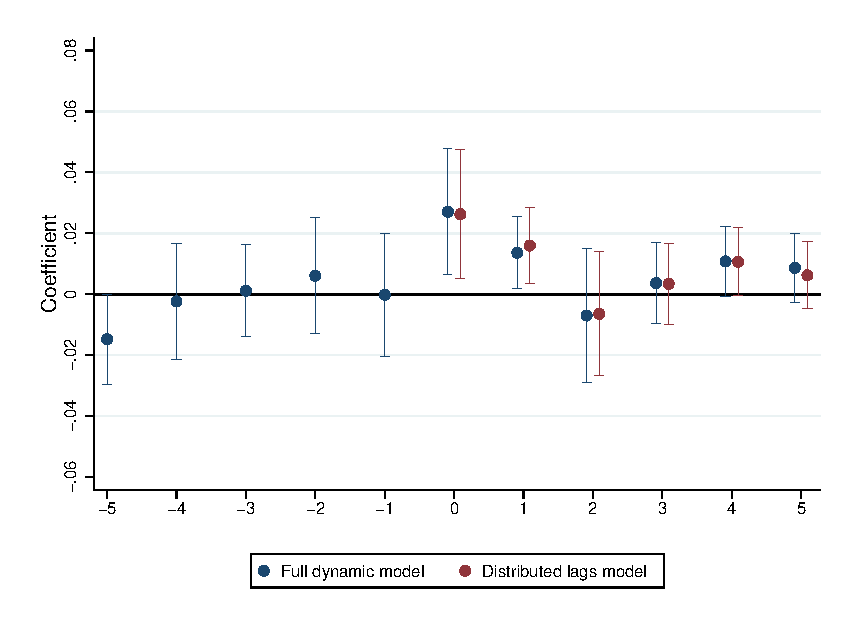
\includegraphics[width = \textwidth]
		{../../analysis/first_differences/output/fd_models_coeffs_w5.eps}
	\end{subfigure}
	\begin{subfigure}[b]{0.8\textwidth}
		\caption{Cumulative sum}
		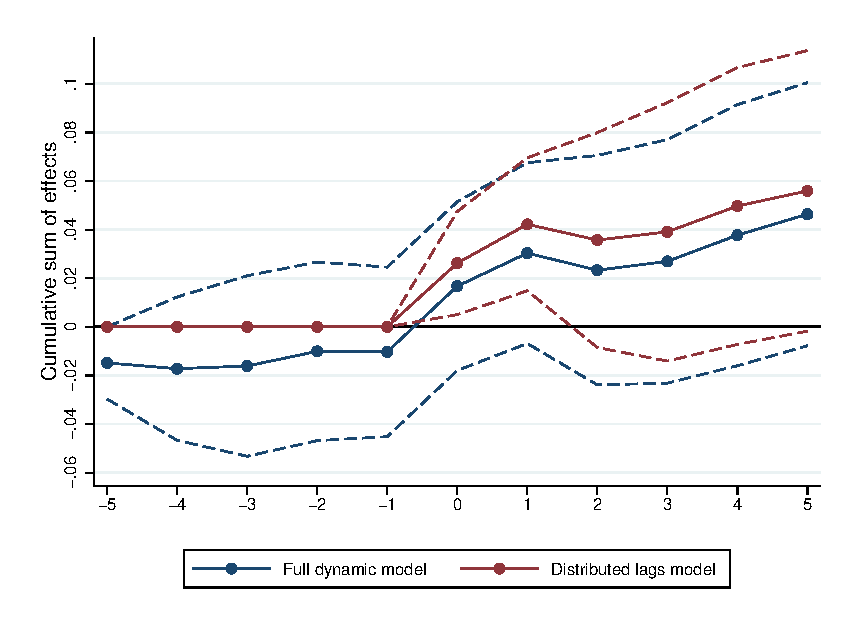
\includegraphics[width = \textwidth]
		{../../analysis/first_differences/output/fd_models_cumsum.eps}
	\end{subfigure}
\end{figure}


\clearpage
\begin{figure}[htb!]
	\caption{Dynamic model: changing window}
	\centering
	\begin{subfigure}[b]{0.5\textwidth}
		\caption{$w=3$}
		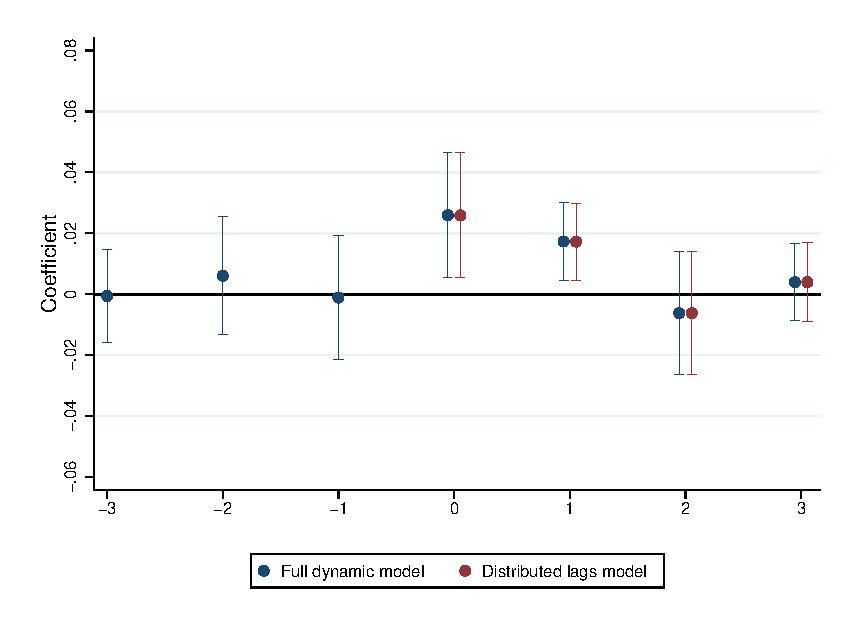
\includegraphics[width = \textwidth]
		{../../analysis/first_differences/output/fd_models_coeffs_w3.eps}
	\end{subfigure}%
	\begin{subfigure}[b]{0.5\textwidth}
		\caption{$w=6$}
		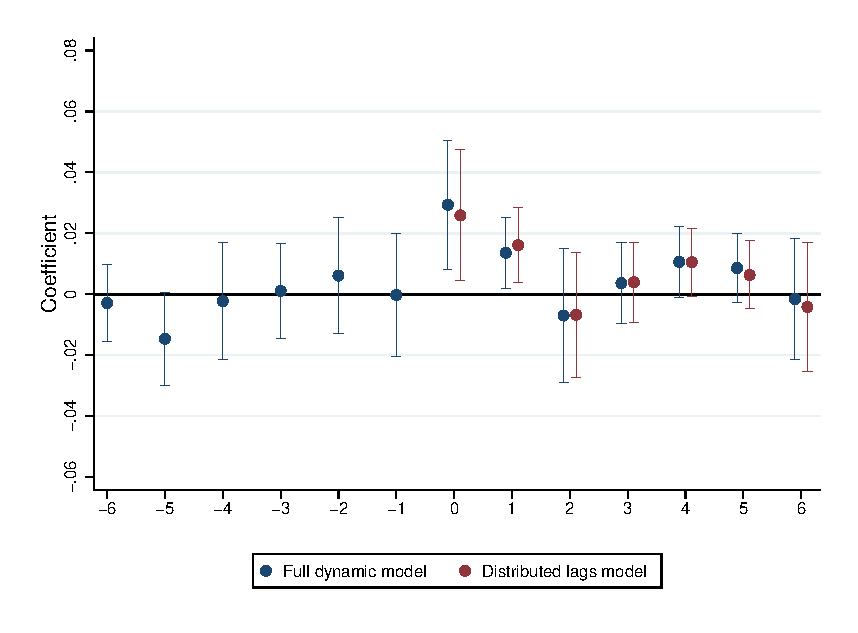
\includegraphics[width = \textwidth]
		{../../analysis/first_differences/output/fd_models_coeffs_w6.eps}
	\end{subfigure}\\
	\begin{subfigure}[b]{0.5\textwidth}
		\caption{$w=9$}
		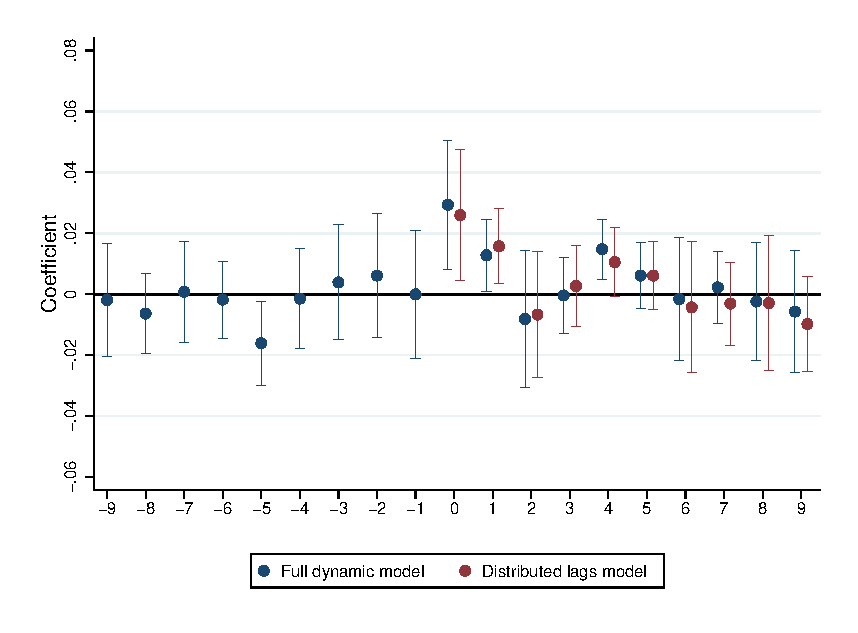
\includegraphics[width = \textwidth]
		{../../analysis/first_differences/output/fd_models_coeffs_w9.eps}
	\end{subfigure}
\end{figure}

\begin{figure} \centering
	\caption{Dynamic model: varying controls}
	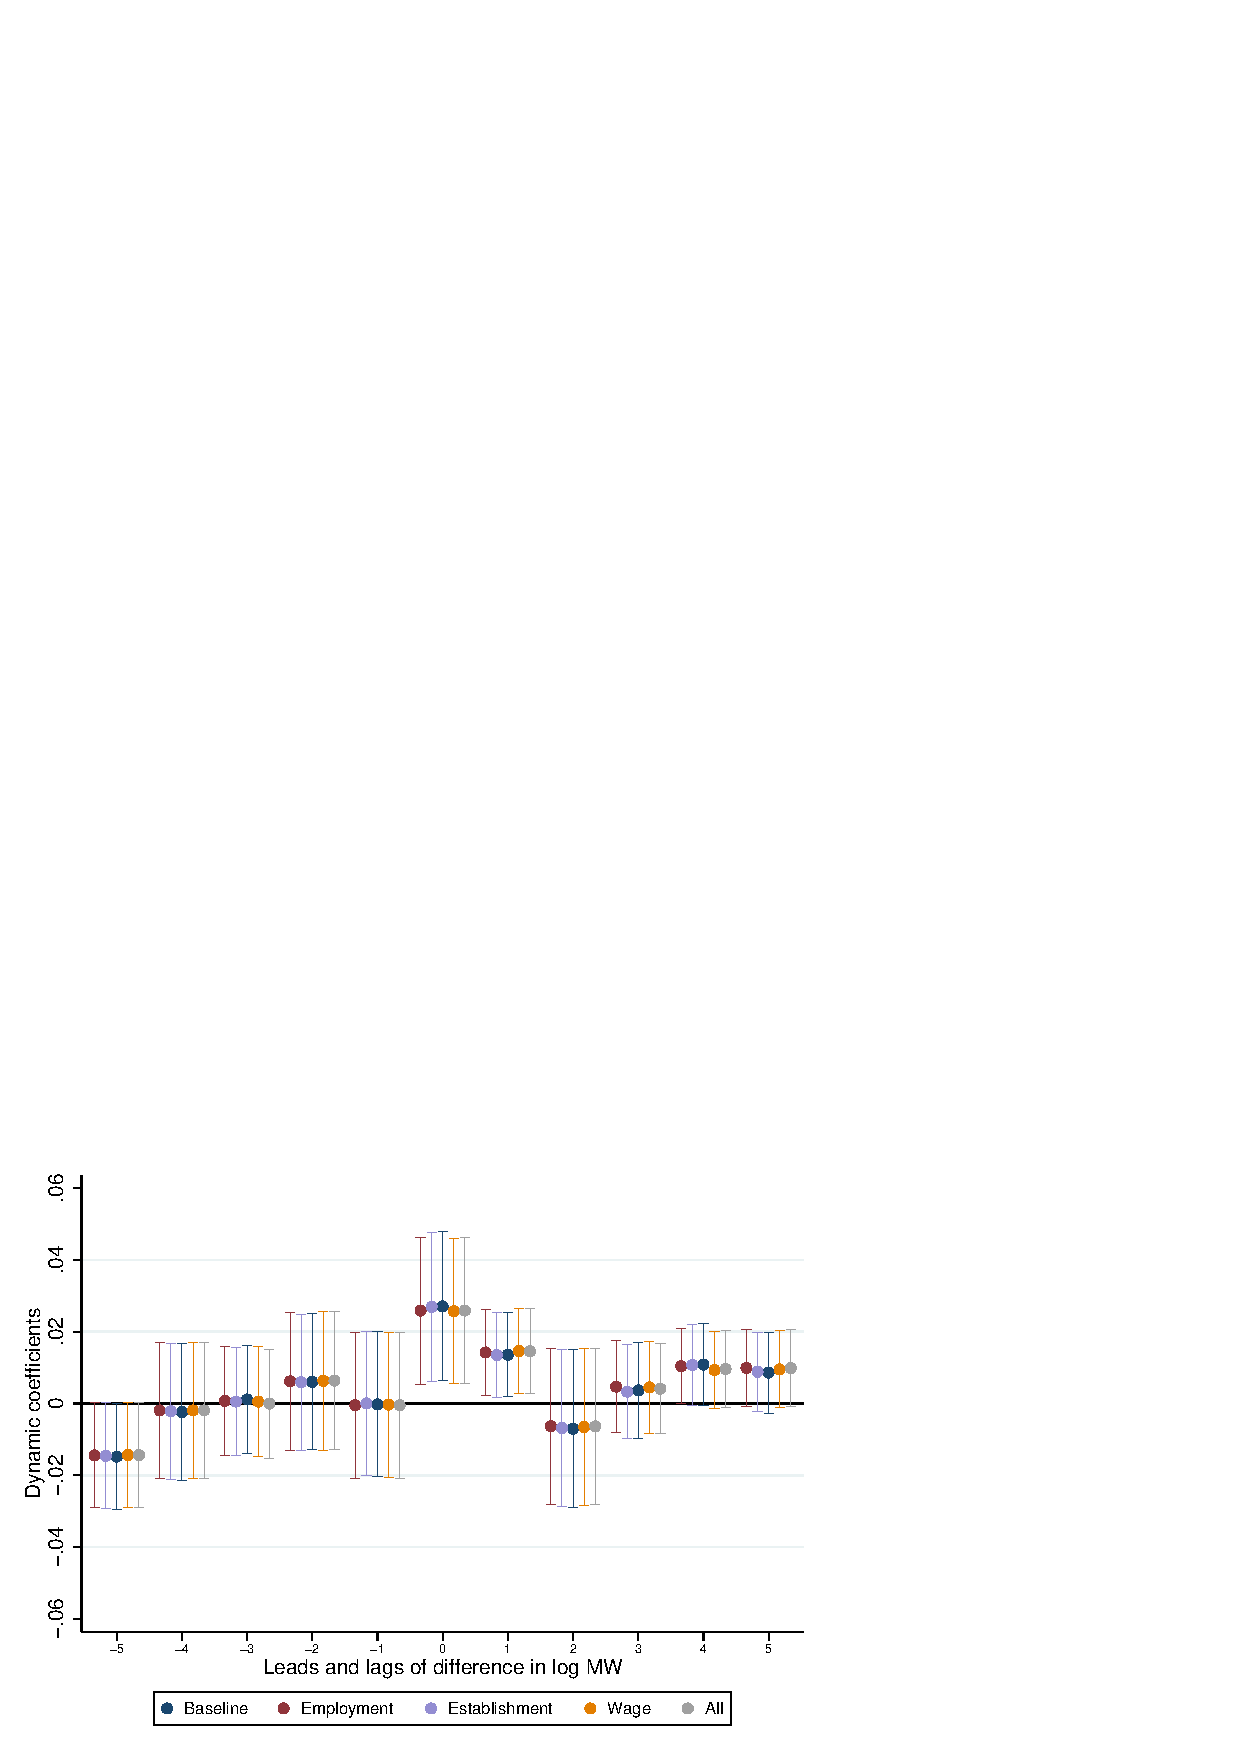
\includegraphics[width = 0.8\textwidth]{../../analysis/first_differences/output/fd_models_control.png}
\end{figure} 

\clearpage
\begin{figure}
	\centering
	\caption{Comparison Between Zillow Sample and Population Density in CBSAs}
	\begin{subfigure}[b]{\textwidth}
		\includegraphics[width = \textwidth]{../../analysis/descriptive/output/sample_map.png}
	\end{subfigure}
	\quad 
	\begin{subfigure}[b]{\textwidth}
		\includegraphics[width = \textwidth]{../../analysis/descriptive/output/popurban_density_map.png}
	\end{subfigure}
\end{figure}

\clearpage 
\begin{figure}\centering
	\captionsetup[subfigure]{justification=centering}
	\caption{Comparison Between Statutory and Experienced Minimum Wage Change for the Seattle MSA}
		\begin{subfigure}[b]{.8\textwidth}
		\centering
		\includegraphics[width = \textwidth]{../../analysis/descriptive/output/Seattle_mw_msa.png}
		\caption{Statutory Minimum Wage}
	\end{subfigure}
	\quad 
	\begin{subfigure}[b]{.8\textwidth}
		\centering
		\includegraphics[width = \textwidth]{../../analysis/descriptive/output/Seattle_expmw_msa.png}
		\caption{Experienced Minimum Wage}
	\end{subfigure}
\subcaption*{\textit{Note:} Minimum wage date change: 01 January 2019}
\end{figure}
\end{document}